\documentclass{article}
\usepackage[utf8]{inputenc}
\usepackage{graphicx,wrapfig}
\usepackage{textcomp}
\usepackage{subcaption}
\usepackage{geometry}
\usepackage{amsmath}
\usepackage{apacite}
\usepackage{array}
\usepackage[table]{xcolor}
\usepackage{float}
\usepackage{amssymb}
\usepackage{fancyhdr}
\usepackage{listings}
\usepackage{xcolor} 
\usepackage[font=tiny,labelfont=bf]{caption}

\floatstyle{plaintop}
\restylefloat{table}
\renewcommand{\arraystretch}{1.8}

\title{Lesson Planner}
\author{GIS Outreach 2021}
\date{Sophie Kolston}

\begin{document}

\maketitle

\tableofcontents

\setlength{\parindent}{0in} 
\newgeometry{top=2.5cm, bottom=3cm, left=2.5cm, right=2.5cm}


\section{Lesson Objectives}
\subsection{Introduction}
This document serves as a lesson planner for myself and hopefully others. This lesson planner is free for anyone to use with no restrictions, including in a commercial capacity (this does NOT include the data provided). The purpose of the lessons is to introduce the unfamiliar to a GIS environment. We have chosen to use ArcMap (reluctantly, thanks to its ease of use for beginners), but the simple tools and concepts mean this could be delivered using a variety of geospatial applications.

\subsection{Target Audience}
Lessons have been written for a community outreach program aimed at getting more GIS education in high school. The idea is to teach high school teachers the basics of GIS so that they can teach it to their students at varying levels. How well this will work, we don't know. Ideally we at least want to bring the awareness of GIS into high schools as geography teachers were often trained before it become as ubiquitous as it is today. My concern is that most high school teachers focus on social geography where GIS papers were not a priority, so they will not deliver its importance to their students. Hopefully lessons like this can help. \\

With all that being said, these lessons cover the very basics that would be expanded on in a first-year GIS course, so would also be useful to complete by keen students. The teacher should be able to complete the tasks in the lessons once or twice to be equipped to deliver it as a formal class.

\subsection{Rote Lesson Objectives}
These lessons are hopefully crafted in such a way that attendees should leave with the following abilities:
\begin{enumerate}
	\item Understand common GIS file types and ways analysts use to manage said files
	\item The ability to produce digital maps, obeying standard mapping conventions
	\item Use simple geoprocessing tools to analyze an area
	\item Understand the basics of Vector and Raster data
	\item Have the ability to deliver such a lesson to intermediate/high school students
\end{enumerate}
\pagebreak

\section{Part 1: Introduction to a GISystem and Cartography}
\subsection{Preamble}
In part 1, students will digitise the extent, and crater, of Mt Taranaki. They will manipulate some contextual data and then export their map with mapping conventions. \\

This lesson will cover the basic data types we deal with in GIS and how to present them. There will be an introduction to vector and raster data with some tools used in geospatial analysis. I would consider the main part of this lesson to be the understanding of how to get data on to ArcMap and how to display it. Folder connection, geodatabases and so on are needlessly confusing, so it is good to dedicate some time to it all. 

\subsection{Data Overview}
The data for this section is as basic as it gets. If the students like, it would be great for them to obtain their own data to place in the map background - just something basic to cover the concept of data wrangling. For now, we will assume they only have what is provided. All data contained in the lesson are pre-converted to NZGD 2000 (EPSG:2193), and are cropped to the Taranaki Regional Council boundary. 

\begin{table}[h]
\begin{center}
    \begin{tabular}{ | m{4cm} | m{1cm}| m{3.5cm} | m{5cm} | m{1cm} | } 
    \hline
    \cellcolor{red!35!blue!33!green!33!}\textbf{Name/Description} & 
    \cellcolor{red!35!blue!33!green!33!}\textbf{Size} &
    \cellcolor{red!35!blue!33!green!33!}\textbf{Source} &
    \cellcolor{red!35!blue!33!green!33!}\textbf{Learning Objective(s)} &
    \cellcolor{red!35!blue!33!green!33!}\textbf{ID} \\
    \hline
    ArcMap basemap & N/A & ESRI (within ArcMap) & Cartography (context) & 10 \\
    \hline
    NZ primary land parcels & 5MB & LINZ & Vector symbology, cartography & 11 \\
    \hline
    NZ road section geometry & 1MB & LINZ & Cartography (context) & 12 \\
    \hline
    \end{tabular}
\end{center}
\caption{\label{tb_data_1}Data used for Part 1}
\end{table}

\subsection{Instructions}
The first step that we will go through is creating a Folder GeoDatabase for the project. Launch ArcMap, then select File $>$ Save. For this example, we can just save to the Desktop. To access the Desktop folder we will first need to create a folder connection to this directory. Folder connections are ways that ArcMap can create catalogues of available data. Go to File $>$ Add Data $>$ Add Data. Click `New Folder Connection' (see Figure \ref{folderconnection}), then navigate to your data folder. Make sure that the data files are extracted from their zip archives. Select the land parcel and road section data, then select `Add'. \\

\begin{figure}[h]
  \centering
  \caption{Creating a folder connection}
  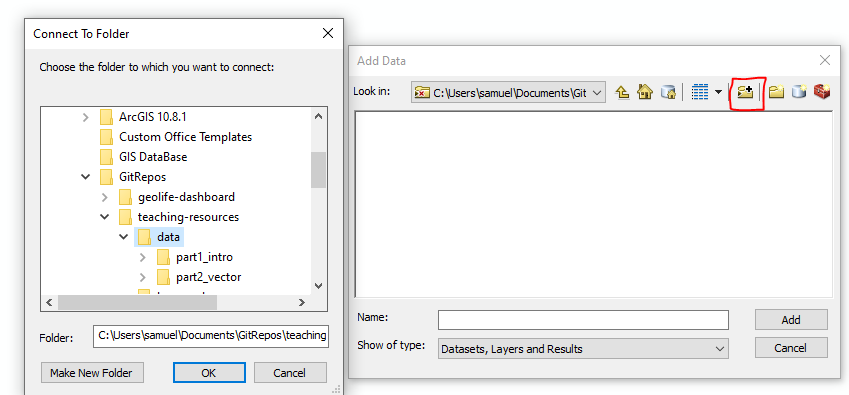
\includegraphics[width=300px]{images/part1/folderconnection.PNG}
  \label{folderconnection}
\end{figure}

The data should now be on the current data frame, and should look something like Figure \ref{rawdata}. We can't really display much information here without showing some background information so that the viewer of the map knows where this is spatially. Select File $>$ Add Data $>$ Add Basemap, and select `NZ Imagery'. We now have imagery of the environment, where it is obvious that we are looking at the Taranaki peninsula. The small checkbox next to each layer of data can enable or disable it.\\

\begin{figure}[h]
  \centering
  \begin{minipage}[b]{0.4\textwidth}
    \centering
    \caption{Our raw data displayed}
    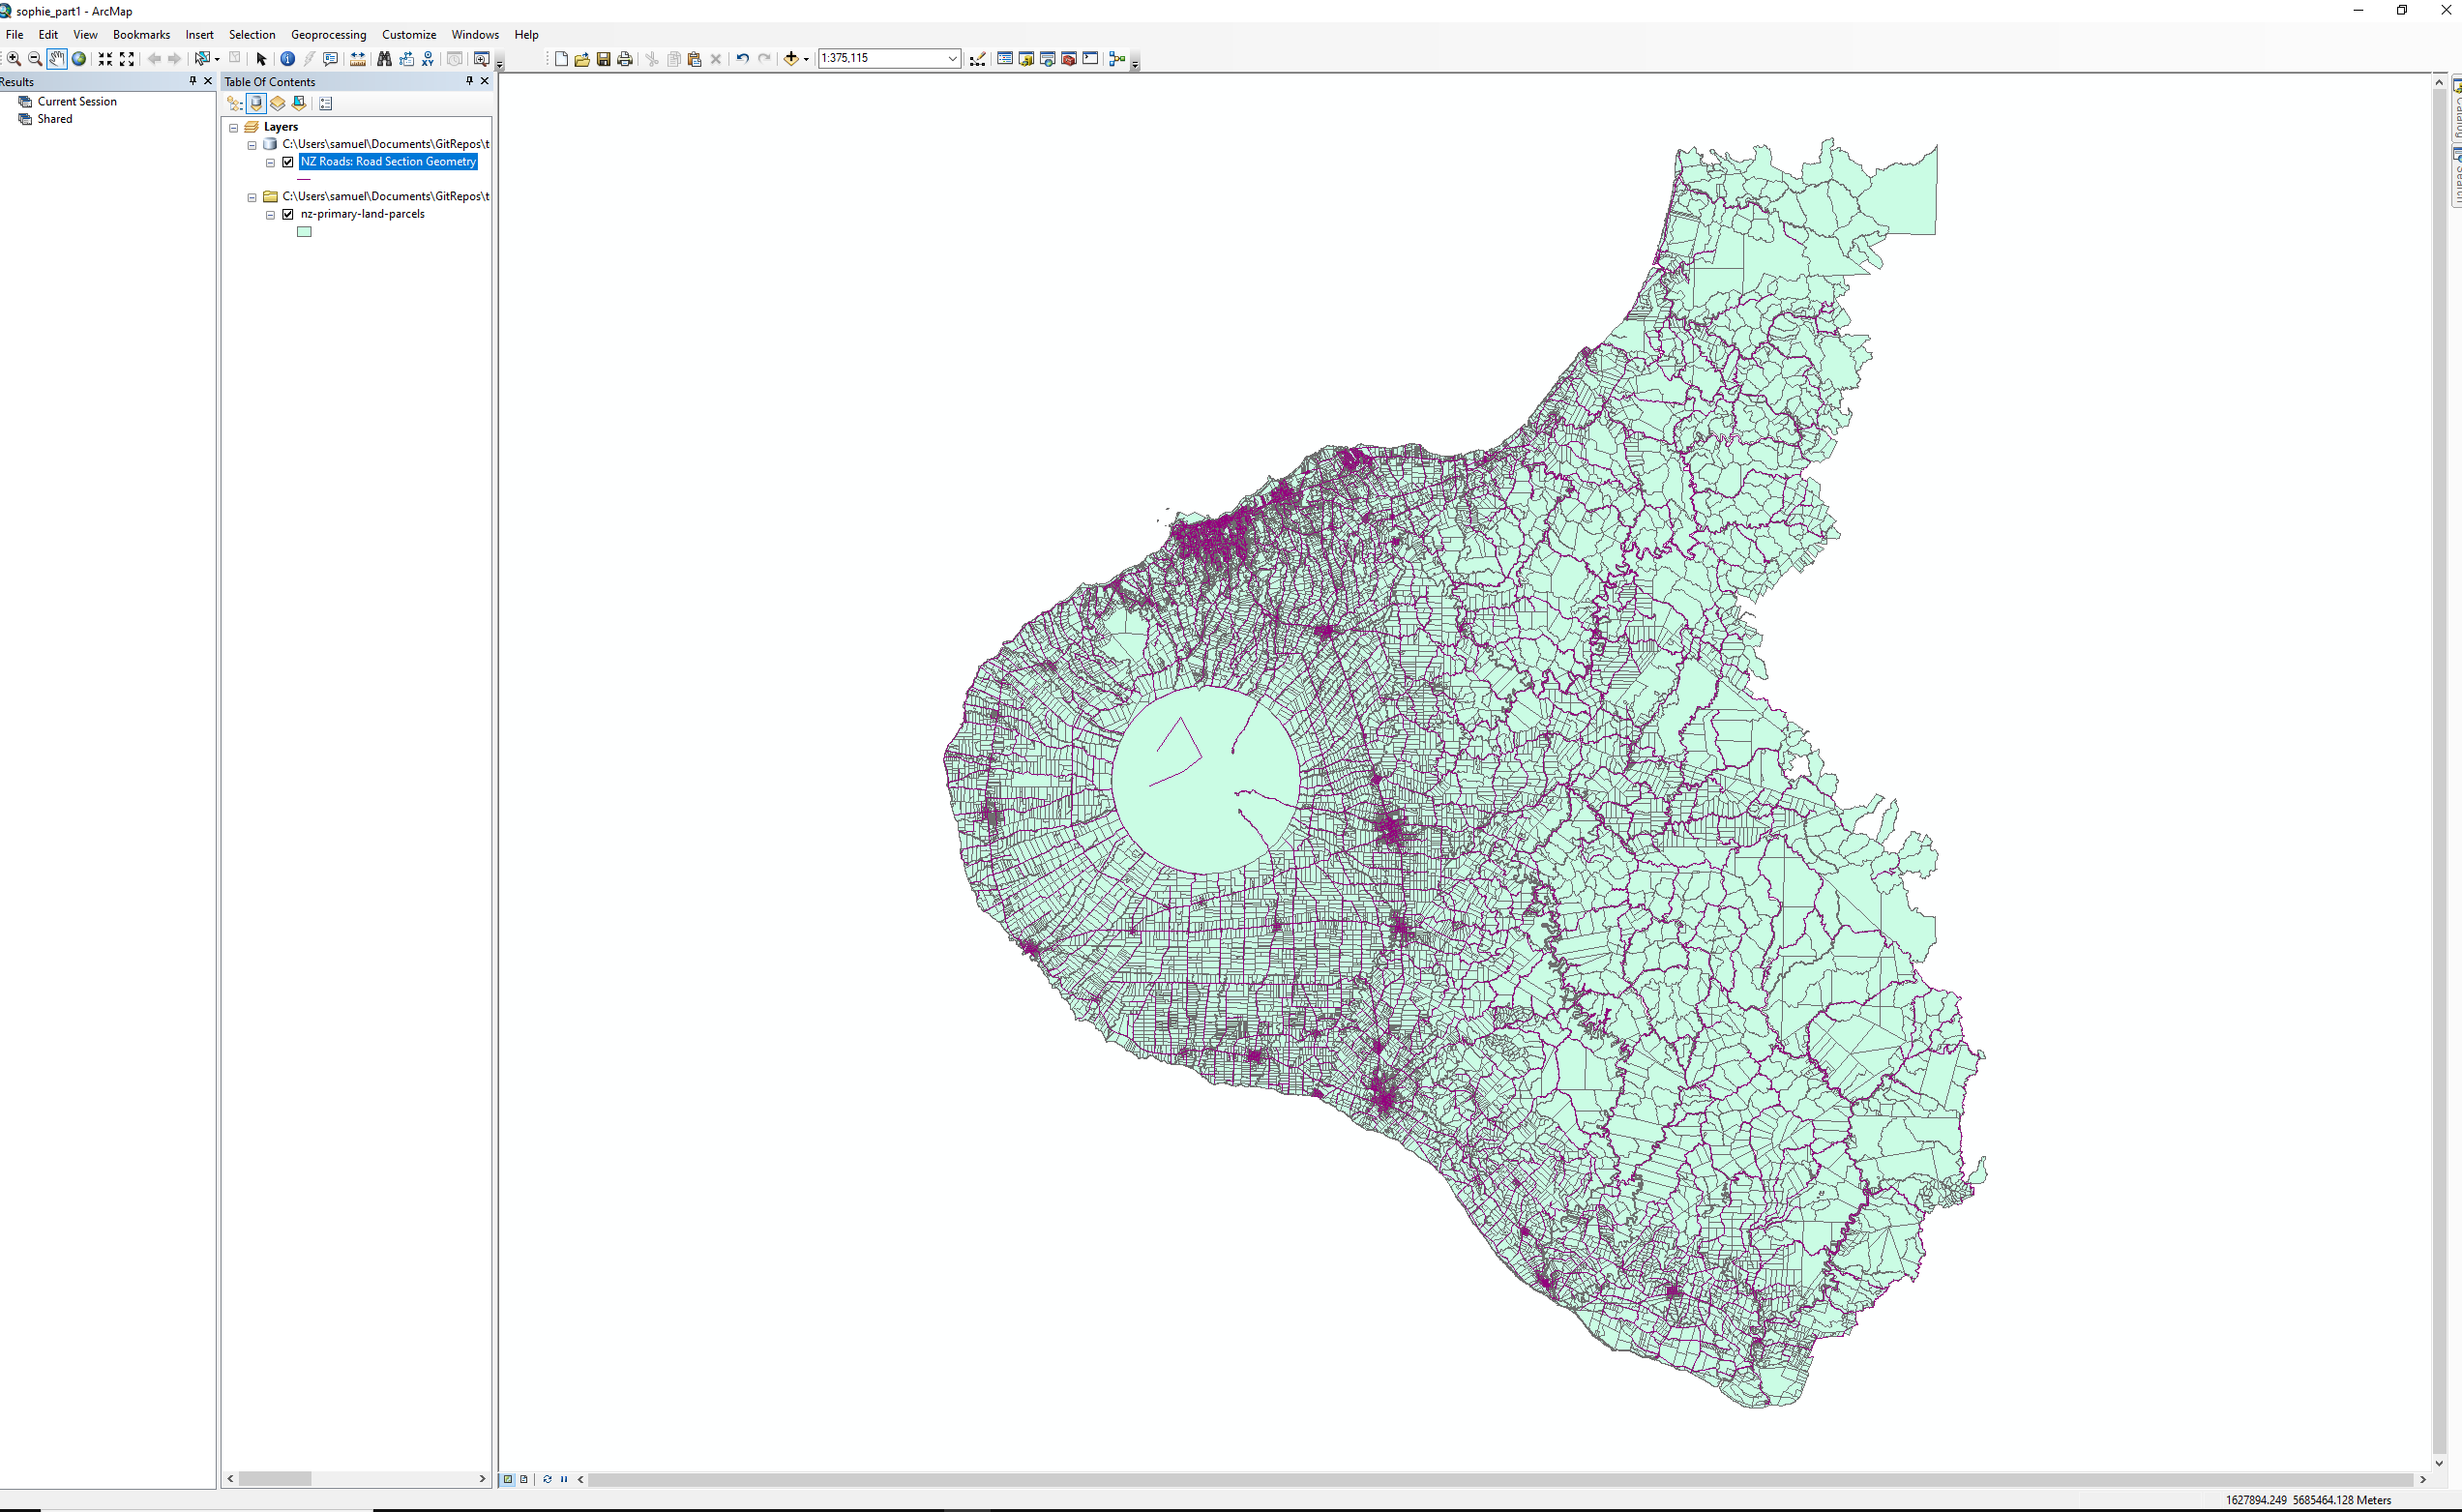
\includegraphics[width=250px]{images/part1/rawdata.PNG}
    \label{rawdata}
  \end{minipage}
  \hfill
  \begin{minipage}[b]{0.4\textwidth}
    \centering
    \caption{Creating a new shapefile}
    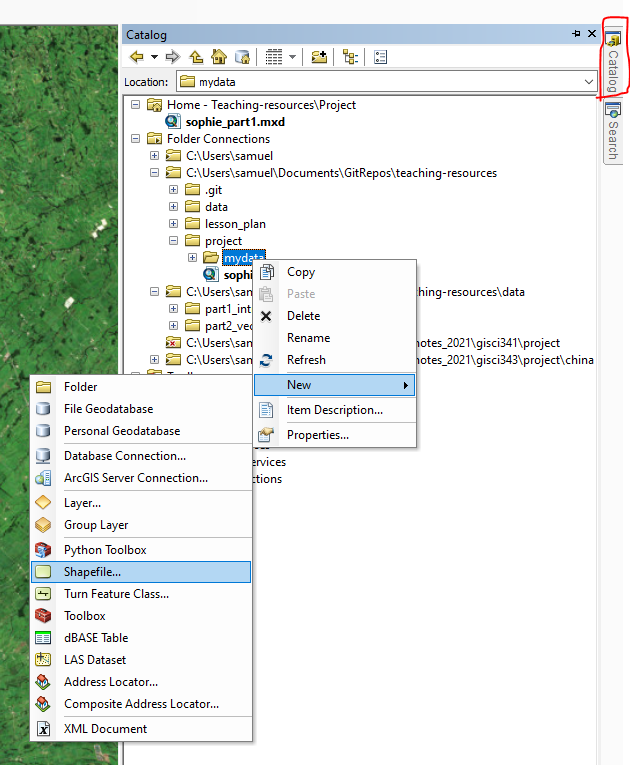
\includegraphics[width=150px]{images/part1/newshp_catalog.PNG}
    \label{newshp_catalog}
  \end{minipage}
\end{figure}

Imagine we have been instructed to digitise the basic geographical features of Mt. Taranaki. To do this, we will draw a polygon around the forested area, as well as a point for the centre point of the mountain. We will need to create a new shapefile to save this data into - select `Catalog' to the right of the screen (see Figure \ref{newshp_catalog}), right click on the folder you would like to save it in $>$ New $>$ Shapefile. Set a relevant name, see Figure \ref{newshp_featurename} for mine, then make the type `Polygon'. Ignore spatial reference for now (as well as the error that will come up). The new file should appear on your list of layers. To add features, we can enable the editing toolbar by clicking Customize $>$ Toolbars $>$ Editor. On the new toolbar that has appeared, click Editor $>$ Start Editing. Select the shapefile you just created (see Figure \ref{newshp_startediting}), then go back to the toolbar and select `Create Features'. We can once again select the shapefile in the new window that has appeared (see Figure \ref{newshp_createfeatures}), and we are finally ready to draw the polygon! Each click with the mouse adds a new vertex to the polygon, and a double-click will end the editing. Draw around the forested area that surrounds Mt. Taranaki (see Figure \ref{newshp_drawingpolygon}), then on the Editor toolbar select Editor $>$ Stop Editing.\\

\begin{figure}[h]
  \centering
  \begin{minipage}[b]{0.4\textwidth}
    \centering
    \caption{Setting the name and type of our new shapefile}
    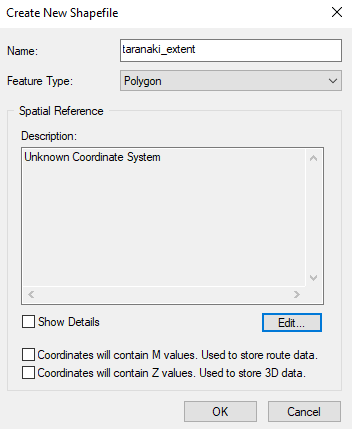
\includegraphics[width=130px]{images/part1/newshp_featurename.PNG}
    \label{newshp_featurename}
  \end{minipage}
  \hfill
  \begin{minipage}[b]{0.4\textwidth}
    \centering
    \caption{Selecting the file to edit}
    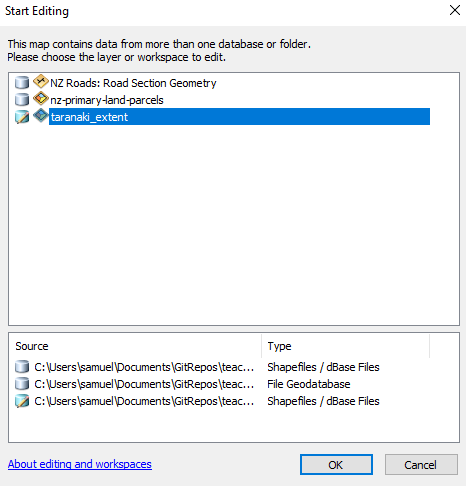
\includegraphics[width=150px]{images/part1/newshp_startediting.PNG}
    \label{newshp_startediting}
  \end{minipage}
\end{figure}
\pagebreak
\begin{figure}[h]
  \centering
  \begin{minipage}[b]{0.4\textwidth}
    \centering
    \caption{Creating features under the editor toolbar}
    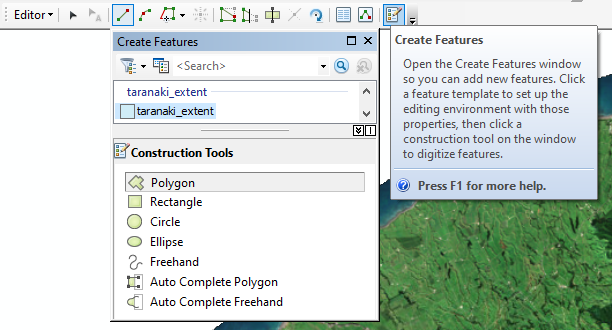
\includegraphics[width=250px]{images/part1/newshp_createfeatures.PNG}
    \label{newshp_createfeatures}
  \end{minipage}
  \hfill
  \begin{minipage}[b]{0.4\textwidth}
    \centering
    \caption{Drawing a polygon around Taranaki}
    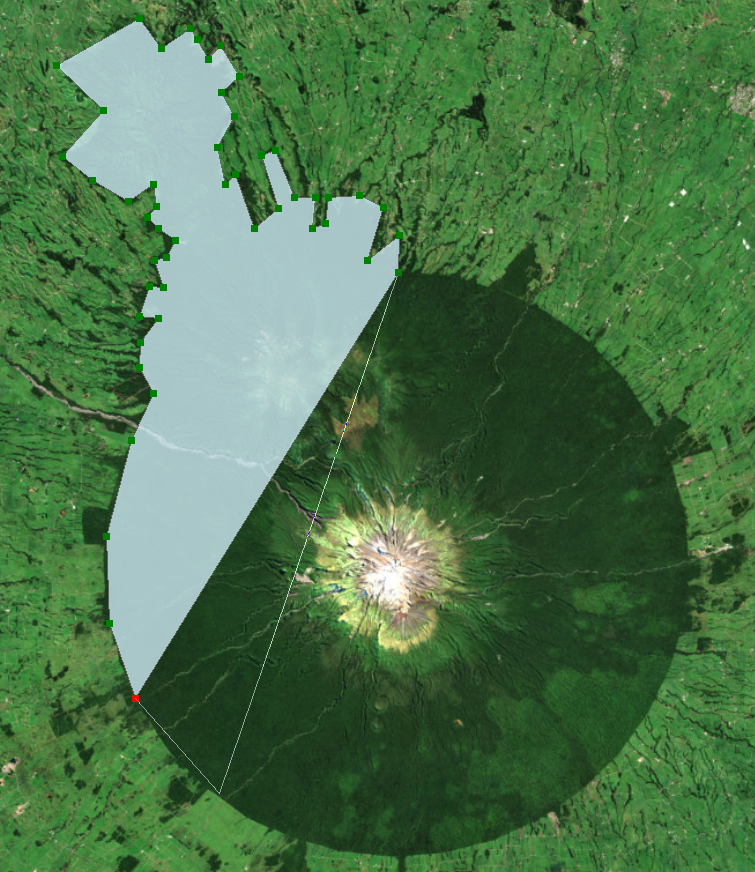
\includegraphics[width=150px]{images/part1/newshp_drawingpolygon.PNG}
    \label{newshp_drawingpolygon}
  \end{minipage}
\end{figure}

You should now have a freshly created polygon that covers the extent of Mt. Taranaki. Now follow the same steps on another shapefile, but this time with a `Point' feature type - this will be the crater centre. Note that you might want to untick the polygon in order to see the imagery so that you can judge where the crater will be.\\

\begin{figure}[h]
    \centering
    \caption{Changing the symbology of a layer}
    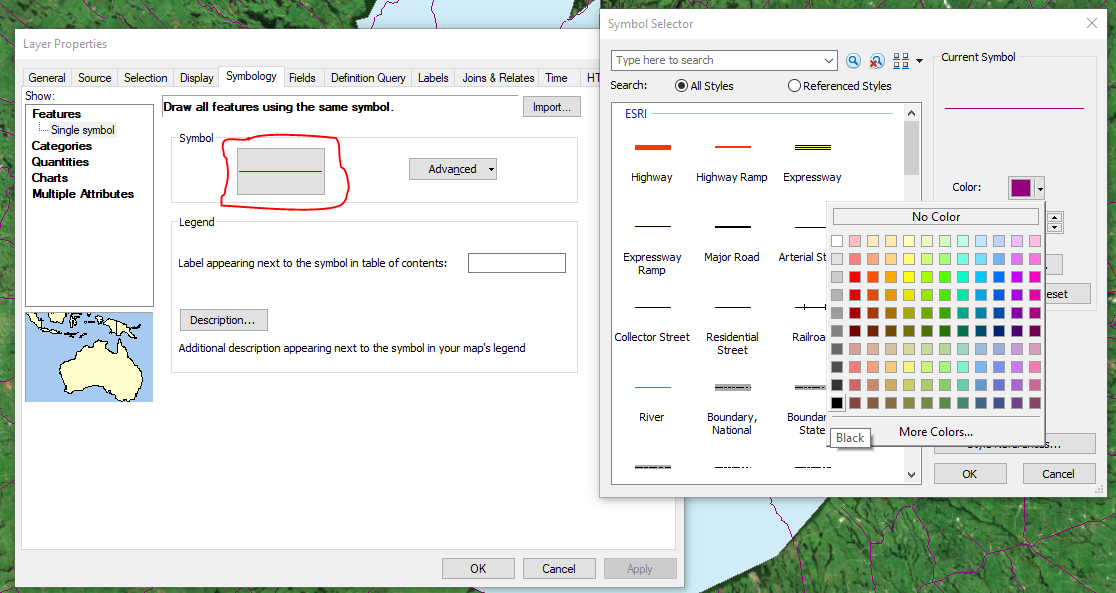
\includegraphics[width=300px]{images/part1/symbology}
    \label{symbology}
\end{figure}

You have successfully created a simple digitisation of a geographic feature. The work in its current form, as an ArcMap project, is not very approachable. Let's create a map so that we can present it. Firstly, we want to add some layers of data for content - these will be the road section and land parcel data we imported earlier. On the roads, right click and select `Properties'. Go to `Symbology' then select the symbol (see Figure \ref{symbology}) and increase the width to 1, with the colour as black. Click `Apply' to save the changes, then close the window and go to the same symbology properties, this time of the land parcel layer. We are going to colour the land parcels based on what type of land they are. To do this, select Categories $>$ Unique Values with the value field as `parcel\_int' (see Figure \ref{symbology_uniquevalues}). This symbology method will colour areas based on a value of an attribute, in this case the use of the land parcel. Select whichever colour ramp you like, save and apply the changes.\\

Next, change the colours and sizing of the extent polygon and crater point so that they are more visible. An important part of cartography is choosing what should be displayed and how - we want a comprise of delivering the most data we can whilst not overwhelming the viewer.
\pagebreak

Lastly, let's adjust the transparency of the land parcels so that we can have a sense of the size and what the features look like underneath. Enable the `Effects' toolbar the same way you did for Editor. Select the land parcel layer in the dropdown (see Figure \ref{transparency}) and increase the transparency to the point where you can see the terrain underneath, but retain the information conveyed by the symbology.\\

\begin{figure}[h]
  \centering
  \begin{minipage}[b]{0.5\textwidth}
    \centering
    \caption{Symbolising our features based on unique values of an attribute}
    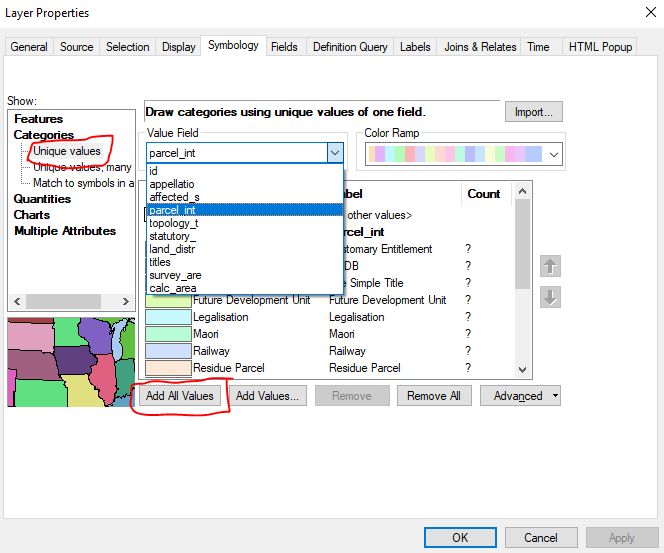
\includegraphics[width=200px]{images/part1/symbology_uniquevalues.PNG}
    \label{symbology_uniquevalues}
  \end{minipage}
  \hfill
  \begin{minipage}[b]{0.4\textwidth}
    \centering
    \caption{Adjusting transparency settings}
    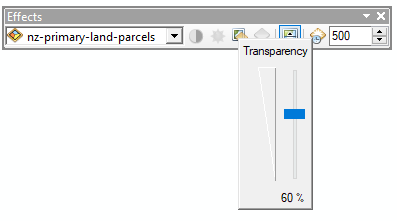
\includegraphics[width=150px]{images/part1/transparency.PNG}
    \label{transparency}
  \end{minipage}
\end{figure}

The processing of data is complete, we are ready to design the map. Select `Layout View' on the bottom left of the map frame (see Figure \ref{layoutview}). Change the page size to A4 landscape by selecting Change Layout $>$ ISO Page Sizes $>$ A4 Landscape (see Figure \ref{layout_changesize}). You can see we now have zoom and pan controls for both the data frame and layout frame. The new controls that have just appeared will control what part of the layout you are looking at, not the data that is displayed. Using `Insert' along the top, add a title and north arrow. I would recommend spending some time looking into the various formatting settings you can make, such as text wrapping and alignment for the title (hint: double-click on the title after creating it). \\

\begin{figure}[h]
  \centering
  \caption{Selecting the Layout view}
  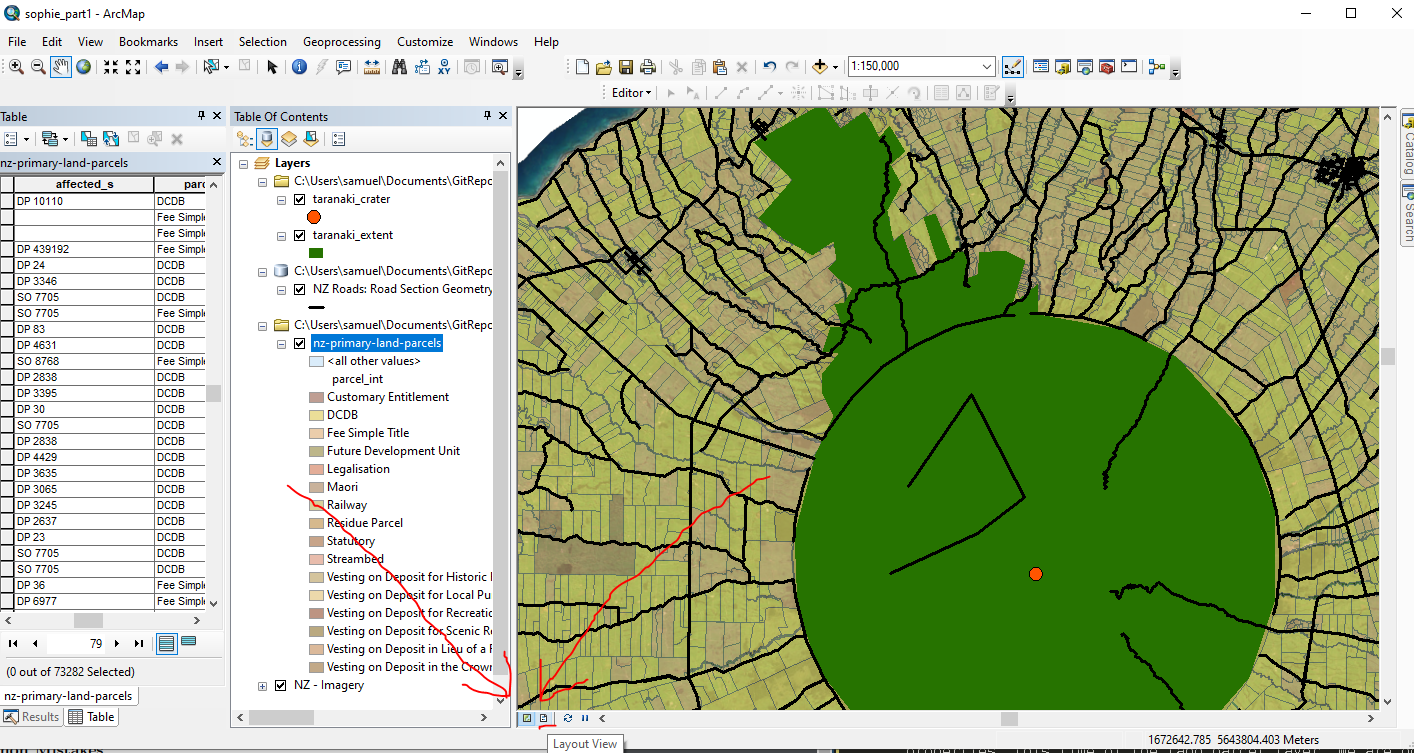
\includegraphics[width=400px]{images/part1/layoutview}
  \label{layoutview}
\end{figure} \pagebreak

\begin{figure}[h]
  \centering
  \begin{minipage}[b]{0.5\textwidth}
    \centering
    \caption{Changing the page size of the layout view}
    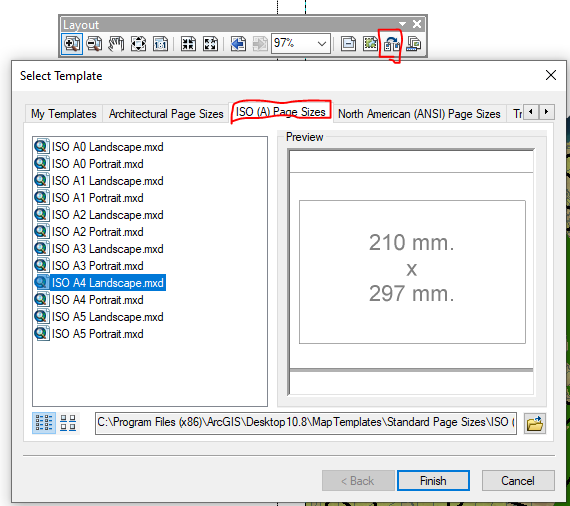
\includegraphics[width=200px]{images/part1/layout_changesize.PNG}
    \label{layout_changesize}
  \end{minipage}
  \hfill
  \begin{minipage}[b]{0.4\textwidth}
    \centering
    \caption{Inserting a legend}
    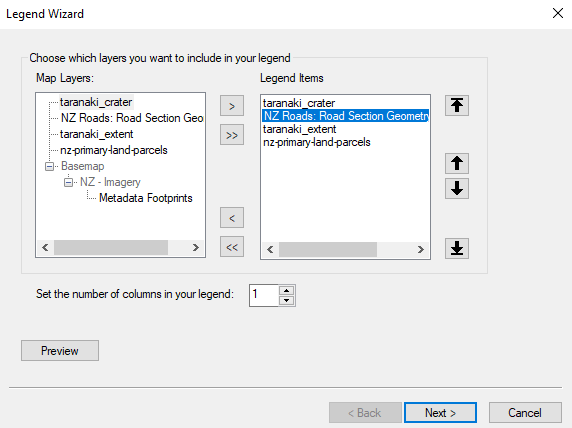
\includegraphics[width=180px]{images/part1/layout_legend.PNG}
    \label{layout_legend}
  \end{minipage}
\end{figure}

Next, let's add a legend so that the reader can see what the colours of the land parcels and our added features represent. Insert $>$ Legend will launch the Legend Wizard. Add all of the layers to be included in the legend (see Figure \ref{layout_legend}), then continue through the wizard leaving everything at default settings. Out will pop up a large legend with a lot of issues. The legend designer for ArcMap is not great, so we can just modify everything manually by converting the legend to a graphics item that can be manipulated with ease. Right-click on the newly created legend then select `Convert to Graphics', then right-click again the select `Ungroup'. You can now go through and make precise modifications to the legend where need be. Further ungrouping items will let you double-click on text items to rename them. I have gone through and changed the name of my created polygons, as well as removing legend items that are not discernible - it is all up to your judgement.\\

\begin{figure}[h]
    \centering
    \caption{Inserting a scale bar}
    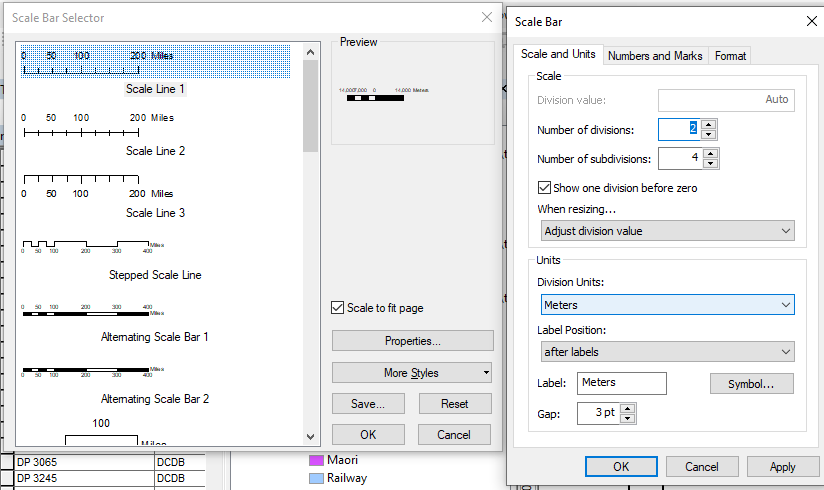
\includegraphics[width=250px]{images/part1/layout_scalebar.PNG}
    \label{layout_scalebar}
\end{figure}

The last cartographic element required is the scale. This shows the distance on the ground relative to the distance on the map, and is an extremely important spatial reference. Insert $>$ Scale Bar will give a lot of design choices, go with whatever you like. Before inserting it, make sure it is in metric and you'll probably want kilometres as a scale reference given the area we are interested in (see Figure \ref{layout_scalebar}).\\

Click File $>$ Export Map and save the map as a .png with a dpi of 300. Figure \ref{example_part1} shows my final map, which should look along the same lines as yours. Congratulations! You have learnt how to add data and present it in a meaningful way spatially.

\begin{figure}[h]
    \centering
    \caption{An example final map for part 1}
    \includegraphics[width=500px]{images/part1/sophie_part1.png}
    \label{example_part1}
\end{figure}

\subsection{FAQ/Common Mistakes}
\begin{itemize}
    \item Make sure the `Spatial Analyst' extension is enabled. Toolbar $>$ Customize $>$ Extensions
    \item Error 999999... Make sure you have no spaces in your file names. I suggest employing `snake case', where spaces are replaced with underscores \_
\end{itemize}

\pagebreak

\section{Part 2: Vector Analysis}
\subsection{Preamble}
In part 2, students will cover the basics of vector analysis. They will work with volcano and census data in Auckland to determine the potential loss of life as the result of the awakening of the Auckland Volcanic Field. \\

The main parts to this lesson are the geoprocessing and familiarity with census data. This section will feature significantly less direct instruction and screenshots than lesson 1, as we can assume a basic understanding of the ArcMap user interface and cartographic convention.

\subsection{Data Overview}
This section will revolve around a dataset of volcanoes in Auckland. We will use census data (2018) to assess the amount of people within each level of danger. These danger levels will be arbitrarily created buffers around each volcano. A coastline dataset will be used to clip to the mainland, which will need to be converted to a polygon. \\

\begin{table}[h]
\begin{center}
    \begin{tabular}{ | m{4cm} | m{1cm}| m{3.5cm} | m{5cm} | m{1cm} | } 
    \hline
    \cellcolor{red!35!blue!33!green!33!}\textbf{Name/Description} & 
    \cellcolor{red!35!blue!33!green!33!}\textbf{Size} &
    \cellcolor{red!35!blue!33!green!33!}\textbf{Source} &
    \cellcolor{red!35!blue!33!green!33!}\textbf{Learning Objective(s)} &
    \cellcolor{red!35!blue!33!green!33!}\textbf{ID} \\
    \hline
    ArcMap basemap & N/A & ESRI (within ArcMap) & Cartography (context) & 10 \\
    \hline
    Auckland volcanoes & 1MB & Global Volcanism Program (Smithsonian) & Geoprocessing & 20 \\
    \hline
    2018 NZ Census data & 18MB & Statistics New Zealand & Geoprocessing, cartography & 21 \\
    \hline
    NZ Coastlines & 5MB & LINZ & Geoprocessing, cartography & 22 \\
    \hline
    \end{tabular}
\end{center}
\caption{\label{tb_data_2}Data used for Part 2}
\end{table}

\subsection{Instructions}
As always, the first step is to download and load all the data required. Add a folder connection as with lesson 1, then load the volcanoes, census data and coastlines. While you're at it, add your basemap of choice. Your map frame should look something like Figure \ref{2_rawdata}.

\begin{figure}[h]
  \centering
  \caption{Loading the data for lesson 2}
  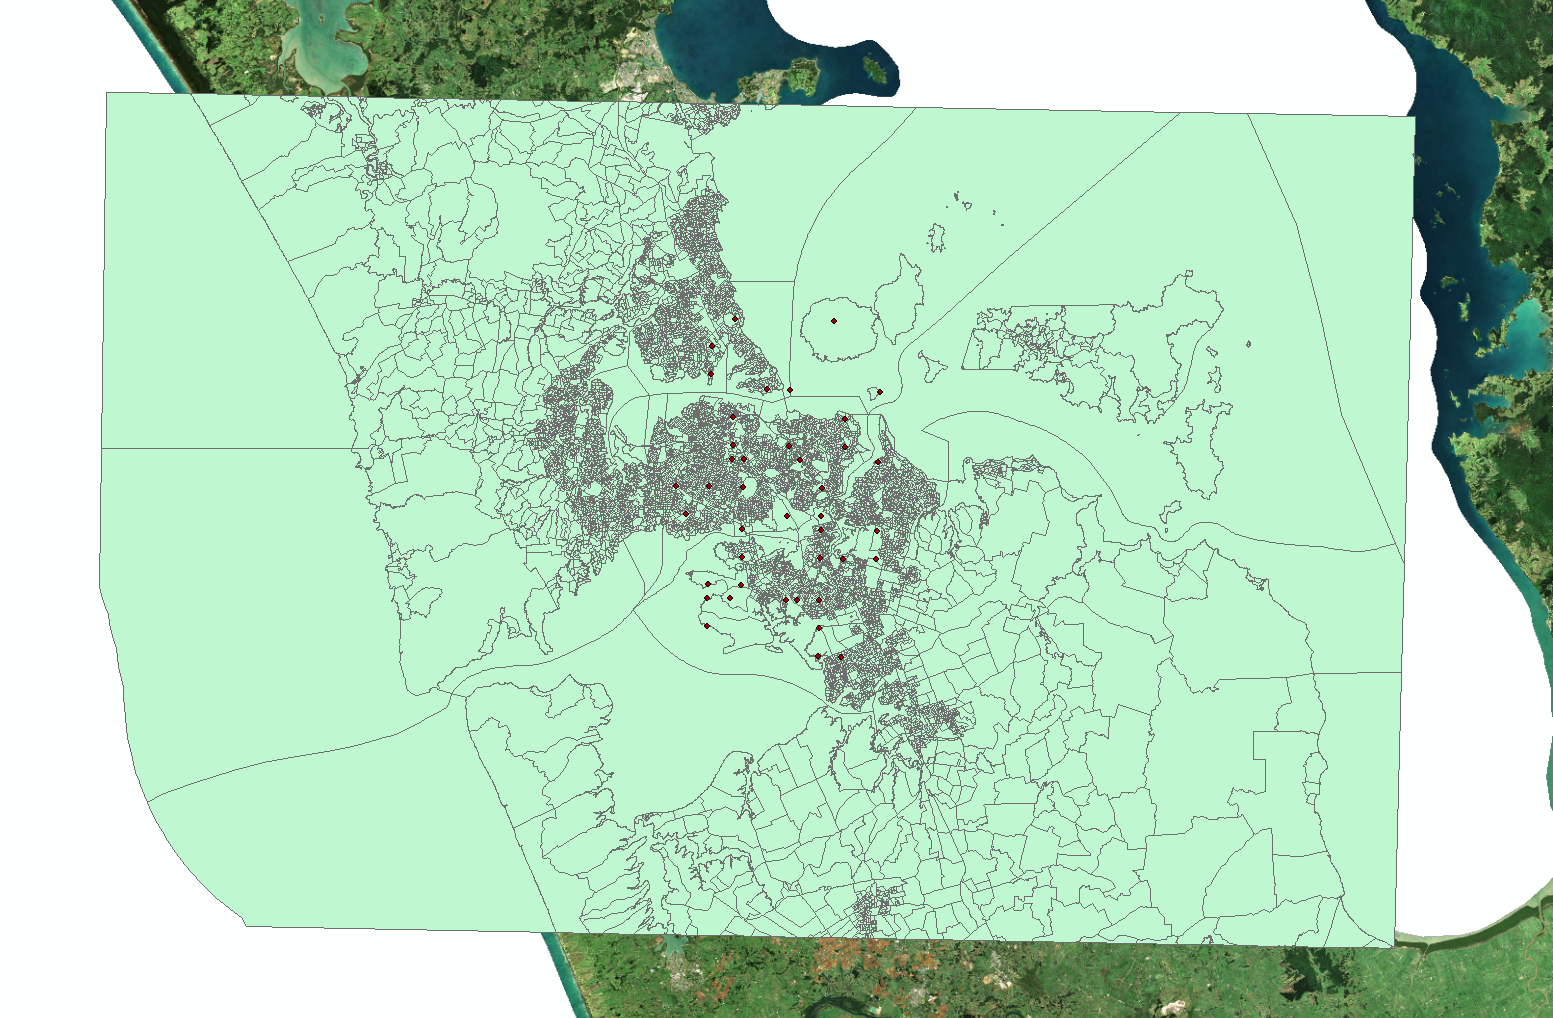
\includegraphics[width=230px]{images/part2/rawdata.PNG}
  \label{2_rawdata}
\end{figure}
\pagebreak

We have the locations of volcanoes within Auckland which we are going to use to create a map of volcanic risk for the region. We are going to create a few areas around the volcano, with the closer to the volcano the higher the level of risk. We can estimate the amount of people reside within these areas using basic spatial analysis tools. First things first, let's create the areas of danger around the volcanoes. To do this, we can use the buffer tool. The buffer tool (see Figure \ref{2_volcanobuffer}) takes an input feature and creates a specified area around it, saving this area as a new feature. You can access the buffer tool by selecting the `Search' window on the right of the main window, and searching for it. The same is true for any geoprocessing tool. Create a buffer of 1000m/1km around the volcanoes layer - I named mine `volcano\_buffer\_1000m.shp'.

\begin{figure}[h]
  \centering
  \caption{Running the buffer tool}
  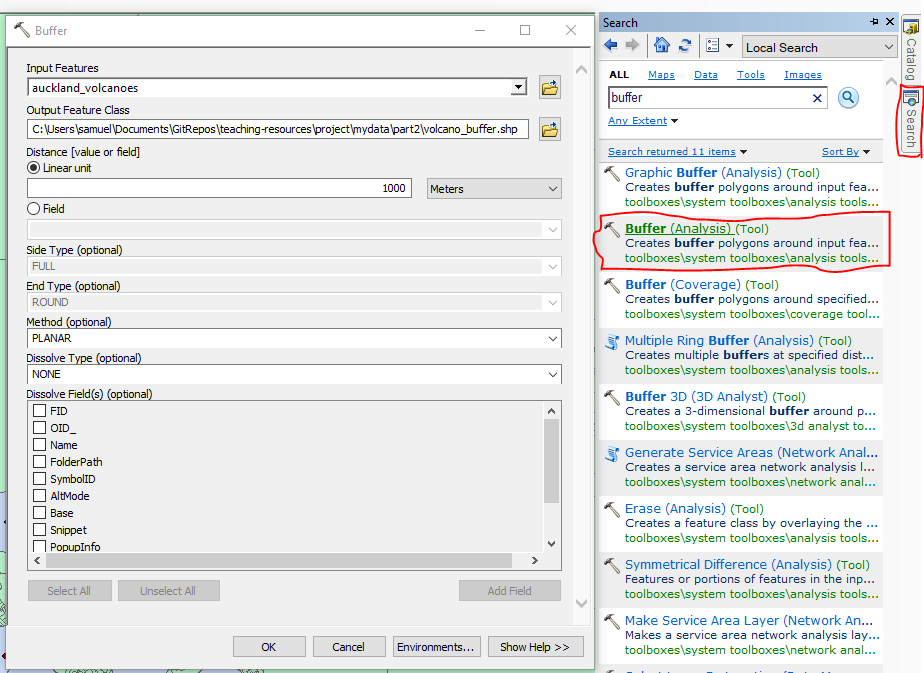
\includegraphics[width=270px]{images/part2/volcano_buffer.PNG}
  \label{2_volcanobuffer}
\end{figure}

The output layer of the buffer should look like Figure \ref{2_buffer_output}. We can see that there are lots of overlapping polygons, where the buffers intersect one another. This can be remedied with the dissolve tool, which aggregates features based on a specified attribute(s). We will be `dissolving' all of the attributes within one layer (the buffer output), so that the overlaps will combine. Run the dissolve tool with the buffer as the input. As can be seen on Figure \ref{2_dissolve}, this tool can be easily found with a quick search. Figure \ref{2_dissolved_output} shows the output, where polygons have been merged together so the overlaps no longer exist.

\begin{figure}[h]
  \centering
  \caption{Running the dissolve tool}
  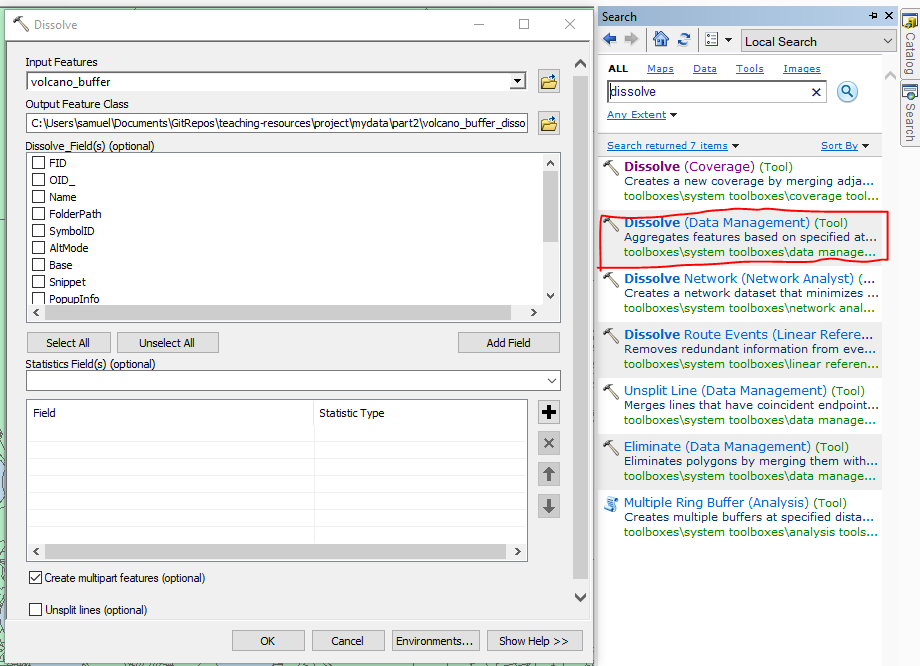
\includegraphics[width=270px]{images/part2/volcano_buffer_dissolved.PNG}
  \label{2_dissolve}
\end{figure}

\pagebreak

\begin{figure}[h]
  \centering
  \begin{minipage}[b]{0.4\textwidth}
    \centering
    \caption{Output of the buffer tool on the volcano layer}
    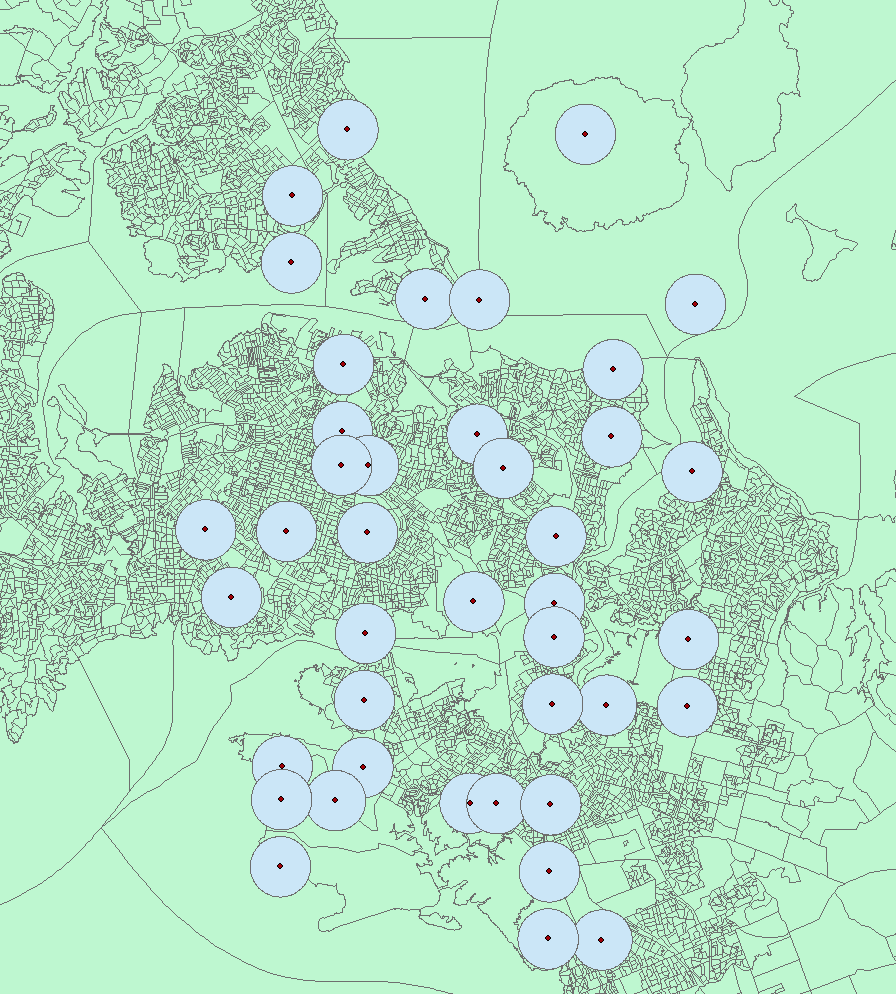
\includegraphics[width=190px]{images/part2/volcano_buffer_output.PNG}
    \label{2_buffer_output}
  \end{minipage}
  \hfill
  \begin{minipage}[b]{0.4\textwidth}
    \centering
    \caption{Output of the dissolve tool on the buffered volcano layer}
    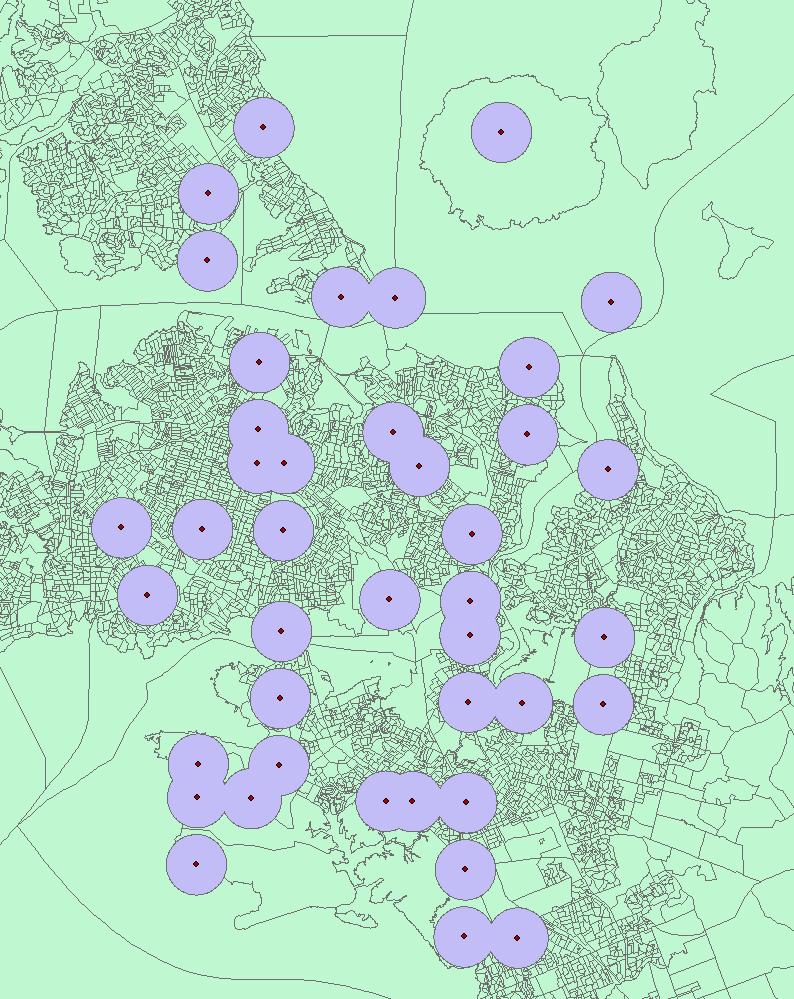
\includegraphics[width=180px]{images/part2/volcano_buffer_dissolved_output.PNG}
    \label{2_dissolved_output}
  \end{minipage}
\end{figure}

Let's see how many people fall within this `high danger' area around the volcanoes of Auckland. There are a few ways to achieve this - something you will find in working with desktop GIS applications is that there are often several ways to tackle a problem. We will use the select by location tool. Go to Selection $>$ Select by Location... (see Figure \ref{2_selectbylocation}), setting the target layer as that of the census, with the dissolved buffer you just created as the source layer. The spatial selection method will be intersect. Click apply, it should look like Figure \ref{2_selection_all}. 

\begin{figure}[h]
  \centering
  \begin{minipage}[b]{0.4\textwidth}
    \centering
    \caption{Selecting by location}
    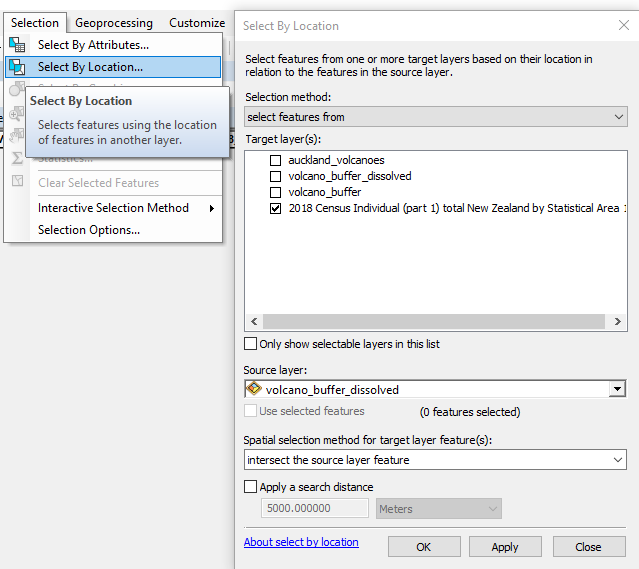
\includegraphics[width=200px]{images/part2/selectbylocation.PNG}
    \label{2_selectbylocation}
  \end{minipage}
  \hfill
  \begin{minipage}[b]{0.4\textwidth}
    \centering
    \caption{Selection from initial select by location}
    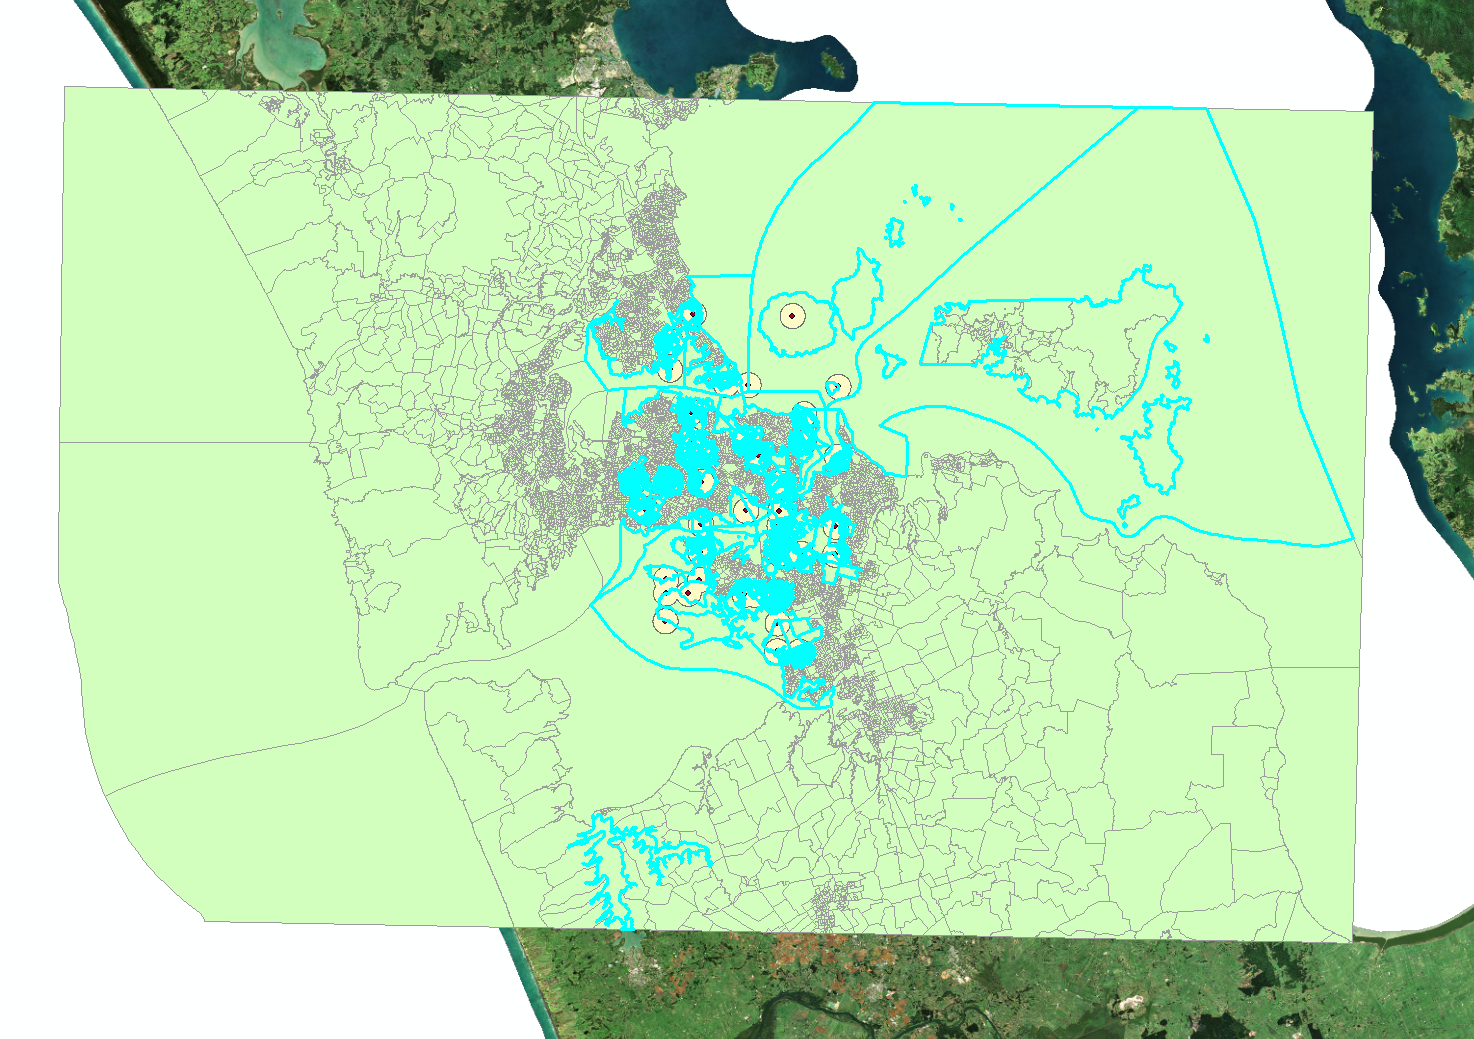
\includegraphics[width=200px]{images/part2/selection_all.PNG}
    \label{2_selection_all}
  \end{minipage}
\end{figure}

That looks a little... off. The census units include offshore islands and the exclusive economic zone around NZ, which we don't really want to factor into our geoprocessing as no people will be full-time residents in these areas. Right-click on the census layer $>$ Open Attribute Table. Here we can see the tabular data that makes up this layer, with the `SHAPE' column containing the geometry, or where the row of data is represented spatially. 
\pagebreak

Following Figure \ref{2_selectbyattributes}, open up the Select by Attributes window. Here we can make a selection within the layer based on a condition(s). Our selection is going to be on the `LANDWATER\_NAME' column, and we want the value to equal to `Mainland'. Running this tool will select all rows that have the value `Mainland' on the specified column, so that we can isolate all areas that are on the mainland. Your map view should look like Figure  (note: make sure you have cleared selected features between steps)

\begin{figure}[h]
  \centering
  \begin{minipage}[b]{0.4\textwidth}
    \centering
    \caption{Select by attributes}
    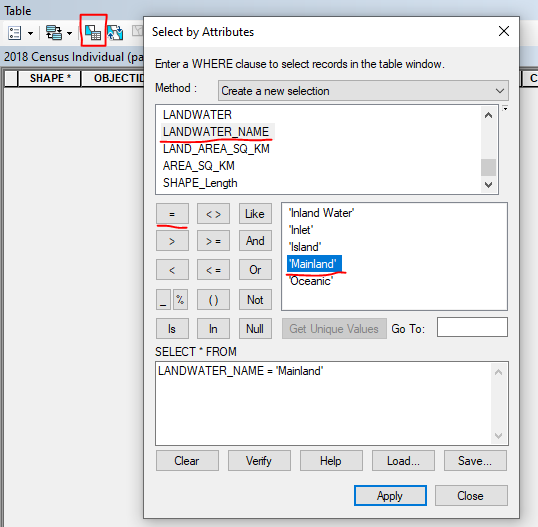
\includegraphics[width=200px]{images/part2/selectbyattributes.PNG}
    \label{2_selectbyattributes}
  \end{minipage}
  \hfill
  \begin{minipage}[b]{0.4\textwidth}
    \centering
    \caption{Selection from select by attributes = mainland}
    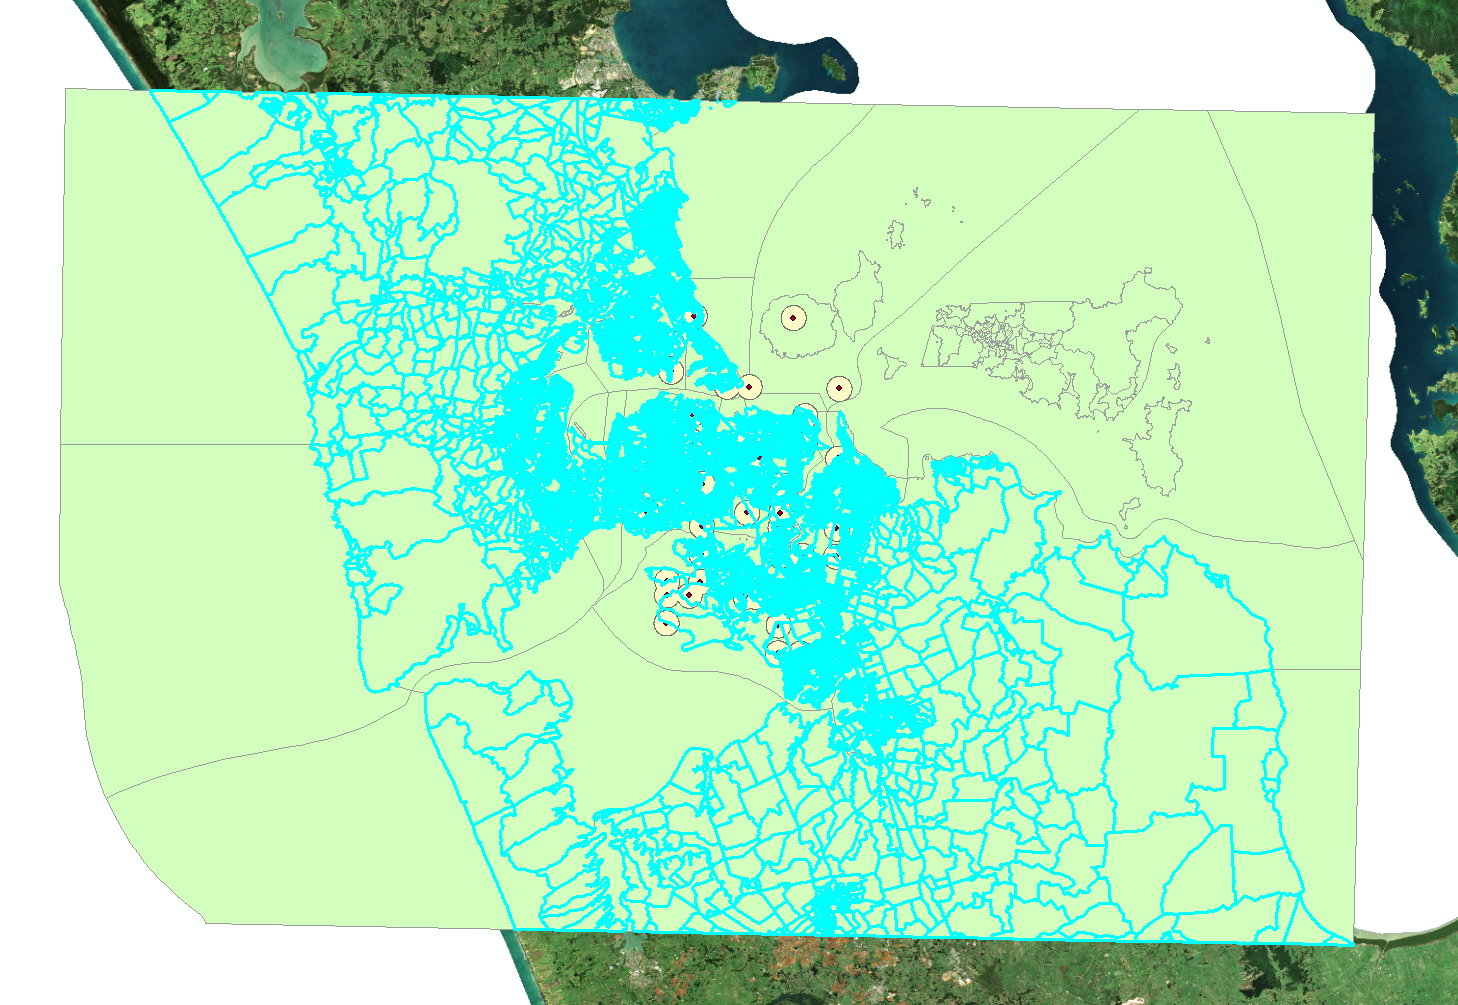
\includegraphics[width=200px]{images/part2/selection_mainland.PNG}
    \label{2_selection_mainland}
  \end{minipage}
\end{figure}

Here we can see we have selected only the areas on land. We want to look at this data only, excluding everything that isn't mainland. Export this selection as its own layer by right-clicking on the census layer $>$ Data $>$ Export Data, leaving the settings as seen on Figure \ref{2_saveselected}. Run the same select by location as you did before, this time with the freshly exported layer as the target layer. The output should only include mainland layers (see Figure \ref{2_selection_mainland_buffer}).

\begin{figure}[h]
  \centering
  \begin{minipage}[b]{0.4\textwidth}
    \centering
    \caption{Saving the current census selection}
    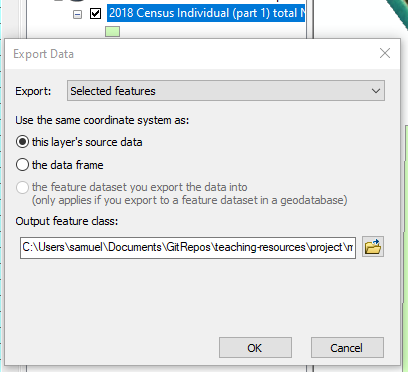
\includegraphics[width=200px]{images/part2/saveselectedfeatures.PNG}
    \label{2_saveselected}
  \end{minipage}
  \hfill
  \begin{minipage}[b]{0.4\textwidth}
    \centering
    \caption{Selection by location of buffer intersecting with census mainland}
    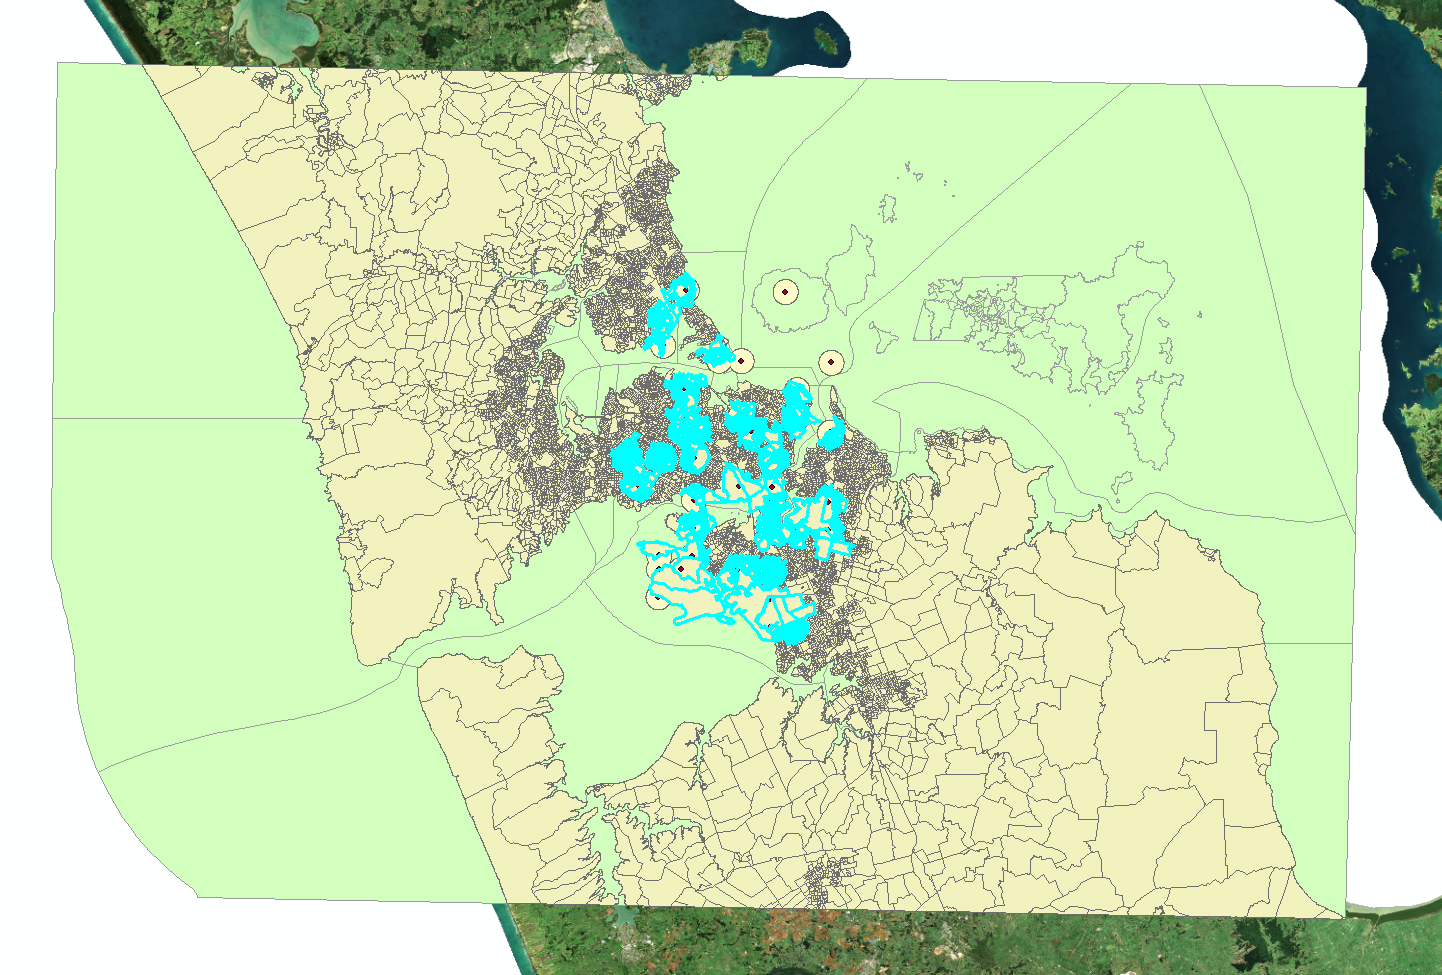
\includegraphics[width=200px]{images/part2/selection_mainland_buffer.PNG}
    \label{2_selection_mainland_buffer}
  \end{minipage}
\end{figure}
\pagebreak

Let's take a look at exactly what this selection is showing. Open up the attribute table of the exported mainland census layer that you have just created a selection on. You can switch the table view to only show selected rows with the small button on the bottom left (see Figure \ref{2_viewattributetable}). Right-click on the column titled `C18\_CURPop' which is the current population of each area as of the 2018 census, then select statistics as per Figure \ref{2_viewattribute_statistics}. You should get a sum of around 280,000. This is the population within our high danger zone area! I encourage you to work out the population that is affected by each of the buffer layers we create. Census population and other demographic information are extremely important to geospatial analysis, so this process is important to be familiar with.

\begin{figure}[h]
  \centering
  \begin{minipage}[b]{0.5\textwidth}
    \centering
    \caption{Viewing selected records on the attribute table}
    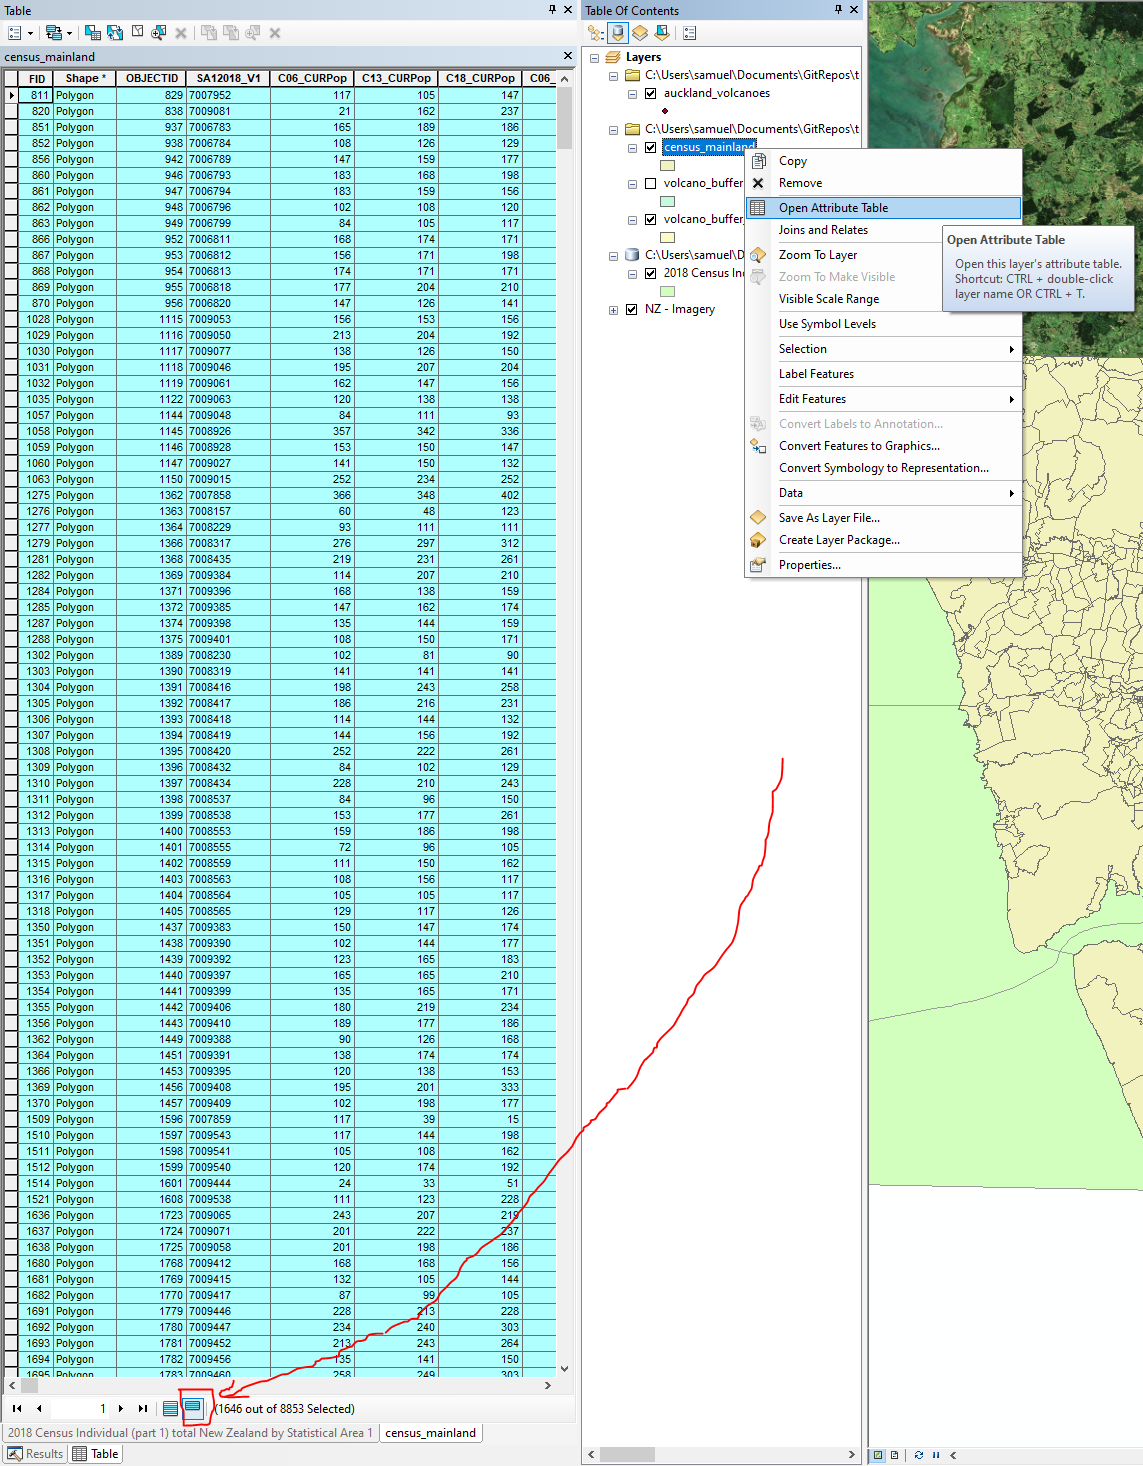
\includegraphics[width=250px]{images/part2/viewattributetable.PNG}
    \label{2_viewattributetable}
  \end{minipage}
  \hfill
  \begin{minipage}[b]{0.4\textwidth}
    \centering
    \caption{Finding the statistics for the selected column}
    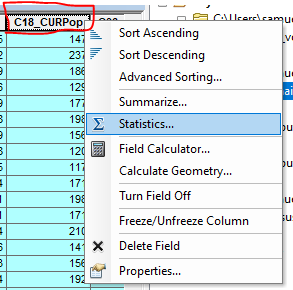
\includegraphics[width=150px]{images/part2/viewattribute_statistics.PNG}
    \label{2_viewattribute_statistics}
  \end{minipage}
\end{figure}

Time to work out other areas of danger. I have defined the areas of danger as 1km, 2.5km and 10km for my analysis. For the purposes of this exercise, you can do whatever you like - I have defined mine arbitrarily. In reality, disaster risk maps like this would be developed with far more rigorous geoprocessing including road network access, underlying lithology, infrastructure pipelines etc. This lesson covers the basics of vector analysis, so we will not go further than these basic tools. All that being said, create two more buffers. Note that the step of manually running the dissolve tool is not neccessary. Figure \ref{2_volcanobuffer_2} shows how the buffer tool can automatically dissolve when running.
\pagebreak

\begin{figure}[h]
  \centering
  \begin{minipage}[b]{0.3\textwidth}
    \centering
    \caption{Buffer tool including a dissolve}
    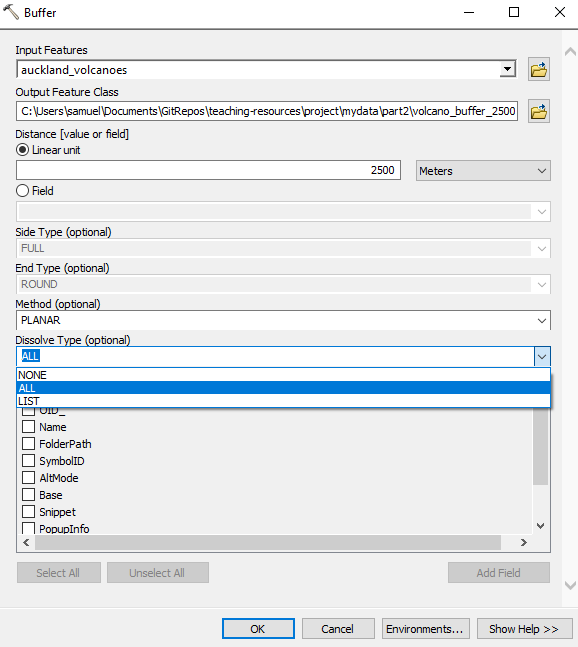
\includegraphics[width=150px]{images/part2/volcano_buffer_2.PNG}
    \label{2_volcanobuffer_2}
  \end{minipage}
  \hfill
  \begin{minipage}[b]{0.5\textwidth}
    \centering
    \caption{Feature to polygon tool on NZ coastline}
    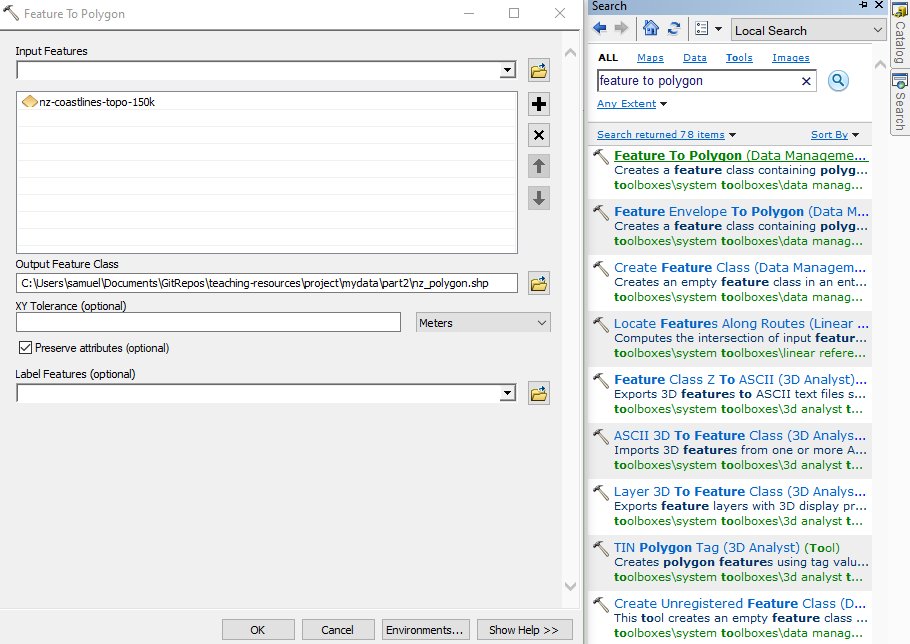
\includegraphics[width=250px]{images/part2/featuretopolygon.PNG}
    \label{2_featuretopolygon}
  \end{minipage}
\end{figure}

feature to polygon tool on coastlines

clip each buffer to nz shapefile

make map

\pagebreak
\section{Part 3: Raster Analysis}
\subsection{Preamble}
\subsection{Data Overview}

\section{Data Sources}
put a bit of a longer description on the data sourced here, and where to find more data in future

\end{document}